\documentclass[a4paper]{report}
\usepackage[utf8]{inputenc}
\usepackage[T1]{fontenc}
\usepackage{RJournal}
\usepackage{amsmath,amssymb,array}
\usepackage{booktabs}


% tightlist command for lists without linebreak
\providecommand{\tightlist}{%
  \setlength{\itemsep}{0pt}\setlength{\parskip}{0pt}}


% Always define CSL refs as bib entries are contained in separate doc
% Pandoc citation processing
\newlength{\cslhangindent}
\setlength{\cslhangindent}{1.5em}
\newlength{\csllabelwidth}
\setlength{\csllabelwidth}{3em}
\newlength{\cslentryspacingunit} % times entry-spacing
\setlength{\cslentryspacingunit}{\parskip}
% for Pandoc 2.8 to 2.10.1
\newenvironment{cslreferences}%
  {}%
  {\par}
% For Pandoc 2.11+
\newenvironment{CSLReferences}[2] % #1 hanging-ident, #2 entry spacing
 {% don't indent paragraphs
  \setlength{\parindent}{0pt}
  % turn on hanging indent if param 1 is 1
  \ifodd #1
  \let\oldpar\par
  \def\par{\hangindent=\cslhangindent\oldpar}
  \fi
  % set entry spacing
  \setlength{\parskip}{#2\cslentryspacingunit}
 }%
 {}
\usepackage{calc}
\newcommand{\CSLBlock}[1]{#1\hfill\break}
\newcommand{\CSLLeftMargin}[1]{\parbox[t]{\csllabelwidth}{#1}}
\newcommand{\CSLRightInline}[1]{\parbox[t]{\linewidth - \csllabelwidth}{#1}\break}
\newcommand{\CSLIndent}[1]{\hspace{\cslhangindent}#1}



\begin{document}


%% do not edit, for illustration only
\sectionhead{Contributed research article}
\volume{14}
\volnumber{3}
\year{2022}
\month{September}
\setcounter{page}{4}

\begin{article}
  % !TeX root = RJwrapper.tex
\title{Editorial}
\author{by Catherine Hurley}

\maketitle


On behalf of the editorial board, I am pleased to present Volume 14 Issue 3 of the R Journal.

\noindent Our incoming editor-in-chief for 2023 Simon Urbanek has been successful in seeking funding from the R Consortium. The project will provide a web-based front-end for managing the R Journal submission and review process.

\noindent Behind the scenes, several people assist with the journal operations. Mitchell O'Hara-Wild continues to work on infrastructure, and thanks to this work, producing a new issue is far more straightforward. H. Sherry Zhang continues to develop the \CRANpkg{rjtools} package under the direction of Professor Dianne Cook. This package, recently available from CRAN assists in producing RMarkdown articles in the R Journal format. In addition, articles in this issue have been carefully copy edited by Hannah Comiskey.

\hypertarget{in-this-issue}{%
\subsection{In this issue}\label{in-this-issue}}

News from the CRAN and Bioconductor are included in this issue.

\noindent This issue features 18 contributed research articles the majority of which relate to R packages
on a diverse range of topics. All packages are available on CRAN. The most common article keywords in this issue are

\begin{center}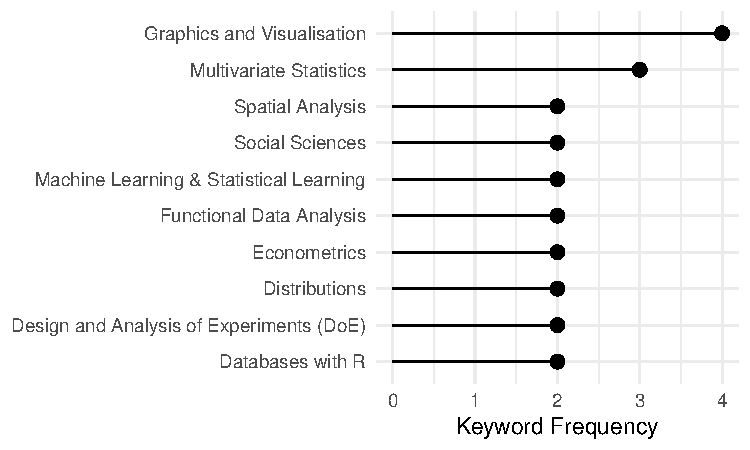
\includegraphics[width=0.5\linewidth]{figs/keywords-1} \end{center}

\noindent For the first time, we give times from submission to article acceptabce for an issue. Median times are just under a year, which is consistent other issues over the last few years.

\begin{center}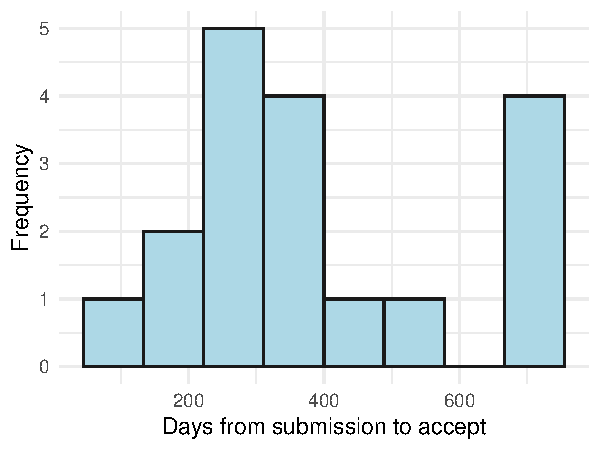
\includegraphics[width=0.5\linewidth]{figs/days-1} \end{center}


\address{%
Catherine Hurley\\
Maynooth University\\%
\\
%
\url{https://journal.r-project.org}\\%
%
\href{mailto:r-journal@r-project.org}{\nolinkurl{r-journal@r-project.org}}%
}

\end{article}


\end{document}
